\documentclass[letter, 10pt]{article}

\usepackage{amsmath}
\usepackage{xcolor}
\usepackage{subfig}
\usepackage[margin = 1in]{geometry}
\usepackage{graphicx}
\usepackage{epstopdf}
\usepackage{pxfonts}
\usepackage{setspace}
\usepackage{titlesec}
\usepackage{booktabs}
\usepackage{fancyhdr}
\usepackage{listings}
\usepackage{multirow}
\usepackage{tikz}
\usepackage{ragged2e}
\usepackage{hyperref}
\usepackage{mathtools}
\usepackage{enumitem}

\usetikzlibrary{positioning}
\usetikzlibrary{fit}

\definecolor{evolotus-color}{RGB}{56,64,96}

\titlespacing{\section}{0pt}{\baselineskip}{0.5\baselineskip}
\titleformat{\section}{\normalfont\fontsize{14}{0}\bfseries}{\thesection}{1em}{}
\titlespacing{\subsection}{0pt}{\baselineskip}{0.2\baselineskip}
\titleformat{\subsection}{\normalfont\fontsize{12}{0}\bfseries}{\thesubsection}{1em}{}
\def\helv{\fontfamily{phv}\bfseries\selectfont}

% http://texblog.net/latex-archive/uncategorized/matrix-align-left-right/
\makeatletter
\renewcommand*\env@matrix[1][c]{\hskip -\arraycolsep
  \let\@ifnextchar\new@ifnextchar
  \array{*\c@MaxMatrixCols #1}}
\makeatother

\begin{document}
\begin{onehalfspacing}

\begin{titlepage}

	\noindent
\includegraphics[scale = 0.4]{evolutus-with-text-blue.eps}
	\vspace{25\baselineskip}\vfill
	
	{\noindent\Large\uppercase{16-662 Robot Autonomy}\\[6pt]
	\Huge\uppercase{\bf Project 2B: Report}}\\[6pt]
	
	\noindent Team Evolutus \\
	\noindent William Ku, Yuhan Long, Yu-Te Cheng, Dawei Wang. \vspace{12pt}
	
	\noindent\today\vfill

\end{titlepage}

\pagestyle{fancy}
\lhead{Project 2B}
\rhead{Team Evolutus}

\setlength{\parskip}{0.5\baselineskip}
\RaggedRight
\parindent=2em

\newpage

\section{Stereo Visual Odometry}
\begin{enumerate}[leftmargin=2em,label={\alph*)}]
\item % a
The Harris feature detector function in MATLAB, {\tt detectHarrisFeatures}, was used to extract features in the first pair of stereo images, {\tt left000.jpg} and {\tt right000.jpg}.
\item % b
Figure \ref{feature} shows the stereo correspondences found using MATLAB's {\tt matchFeatures()} function.

\begin{figure}[b!]
	\centering
	\subfloat[Full correspondences.]{\fbox{
		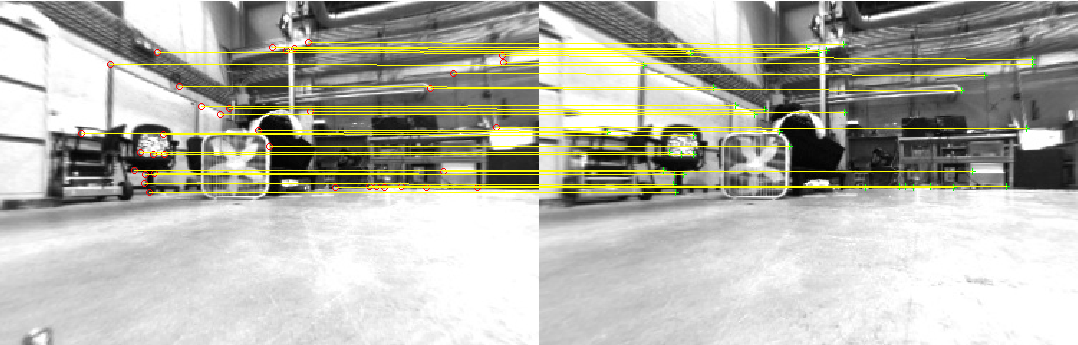
\includegraphics[width = 0.8\textwidth]{feature.png}
		\label{feature}}
	}

	\subfloat[Outliers removed (thick red circle) using RANSAC on reprojection errors.]{\fbox{
		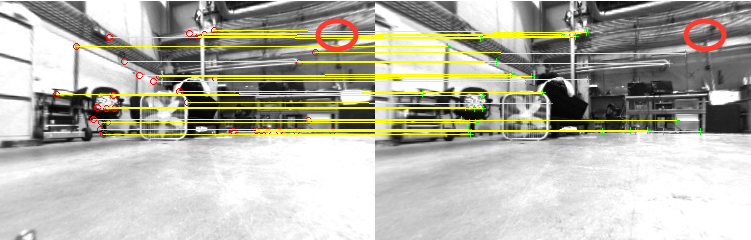
\includegraphics[width = 0.8\textwidth]{featureoutlier.png}
		\label{featureoutlier}}
	}
	\caption{Point correspondences between \texttt{left000.jpg} and \texttt{right000.jpg} using a Harris feature detector.}
\end{figure}

\item % c
Assuming a pinhole camera model, triangulation of the stereo correspondences was performed using Direct Linear Transform (DLT) on the camera projection relation, $x\times PX = 0$, where $P$ is the camera matrix, $X$ the three-dimensional world point, and $x$ the two-dimensional image point of $X$. Plots for the feature locations in Figure \ref{feature} are shown in Figure \ref{3d}.

\begin{figure}[h!]
	\centering
	\subfloat[Front view]{
		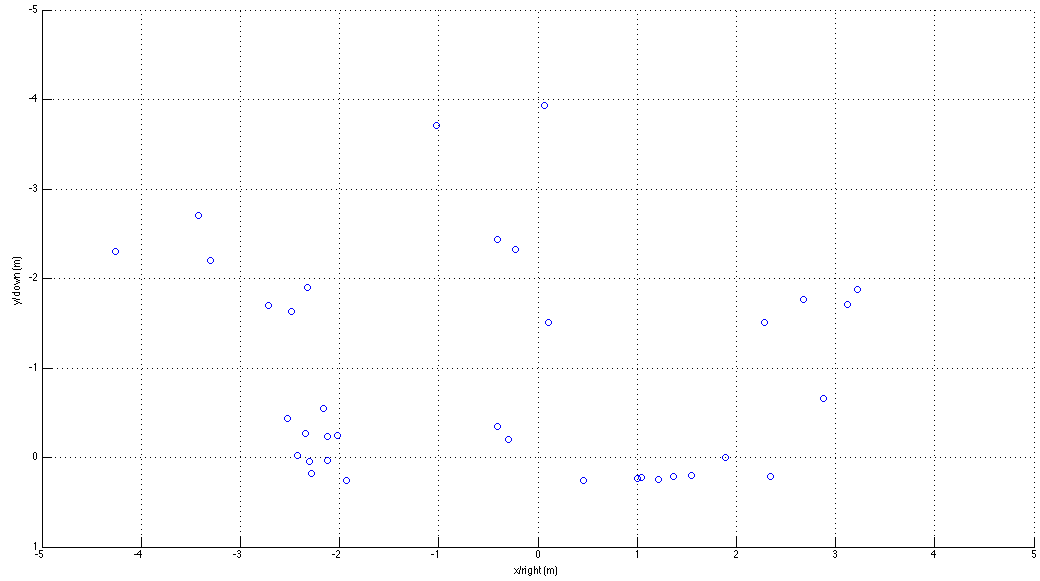
\includegraphics[width=0.4\textwidth]{3dfront.png}
	}
	\subfloat[Top view]{
		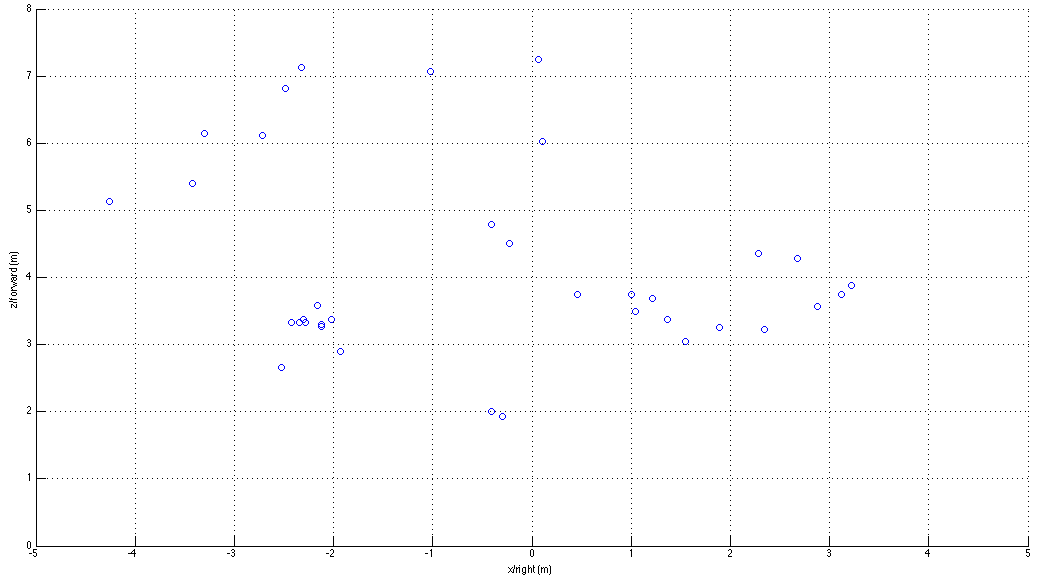
\includegraphics[width=0.4\textwidth]{3dtop.png}
	}
	\caption{The triangulated 3D points of stereo correspondences.}
	\label{3d}
\end{figure}

\item % d
Correspondences between successive left images, \texttt{left000.jpg} and \texttt{left001.jpg} were found using the same feature detection and matching procedure described in parts (a) and (b).

Let $x_n$ and $P_n$ be the correspondence points and the camera matrix for the $n$-th image, then $x_1$ and the 3-D triangulated points, $X$, could be used to estimate the camera matrix, $P_1$ using Direct Linear Transform (DLT). We assume the origin was at the camera center of the previous image, \texttt{left000.jpg} (i.e. $P_0 = K[I_3 | \textbf{0}_3]$, where $K$ is the 3-by-3 upper-triangular camera intrinsic matrix (identical for all images), $I_3$ the 3-by-3 identity matrix, and $\textbf{0}_3$ the 3-by-1 zero vector).

To reject outliers, the computation of $P_n$ was wrapped within a RANSAC routine thresholded by the camera reproduction error, $e = || x_n - P_nX ||$. A minimum of 5.5 such correspondences were needed to compute the 11 degrees-of-freedom for the 3-by-4 camera matrix (minus one for scale ambiguity). For convenience, six correspondences were used for every iteration of the RANSAC procedure. The inlier correspondences are shown in Figure \ref{featureoutlier}.

For the computed camera matrix, $P_n$, the following relationship holds:
\begin{equation}
	P_n = [P_{n, 1-3} | P_{n, 4}]= K[R_n | t_n],
\end{equation}
where $R_n$ and $t_n$ are the rotation and translation between camera frames $n-1$ and $n$. $P_{n, 1-3}$ was decomposed using RQ decomposition to obtain $K$ and $R_n$. Translation was compuled with $t_n = K^{-1}P_{n, 4}$.

\item % e
Parts (a) to (d) were repeated to find $R_n$ and $t_n$ for every successive image pair. Assuming that the camera started at the origin of the world frame, a trajectory, shown in Figure \ref{traj}, was generated by composing sequential transformations of $R_n$ and $t_n$. Note that in Figure \ref{trajfront} the end position falls below the starting position. This will be discussed in a later section. The position and orientation, in ZYX Euler angles, over time are shown in Figures \ref{pos} and \ref{orient}. To increase readability, the $y$ values in all of the position plots in this document were negated due to a downward-pointing y-axis.

\begin{figure}[t]
	\centering
	\subfloat[Front view]{
		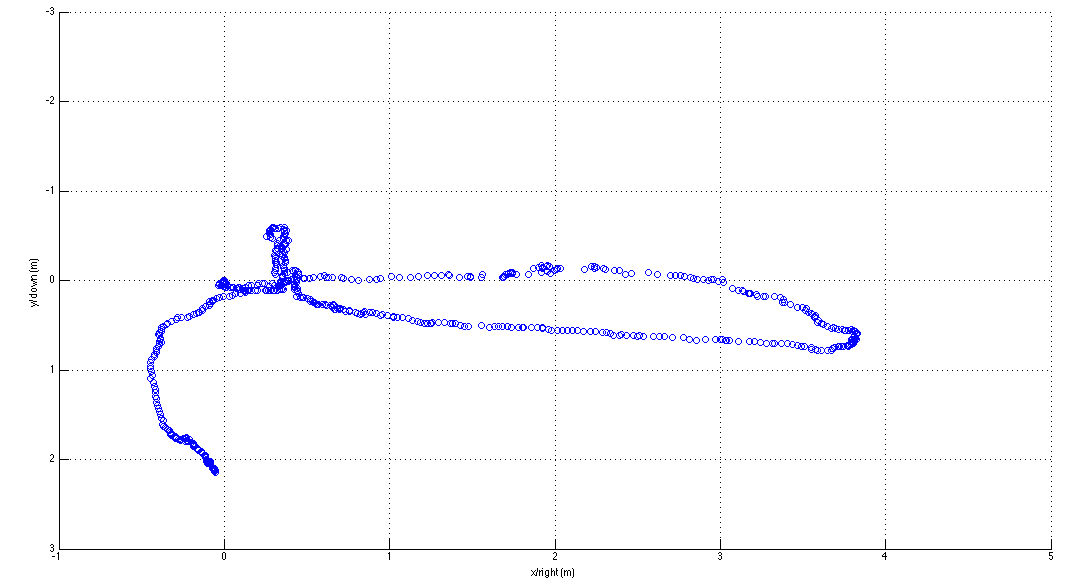
\includegraphics[width=0.4\textwidth]{trajside.png}
		\label{trajfront}
	}
	\subfloat[Top view]{
		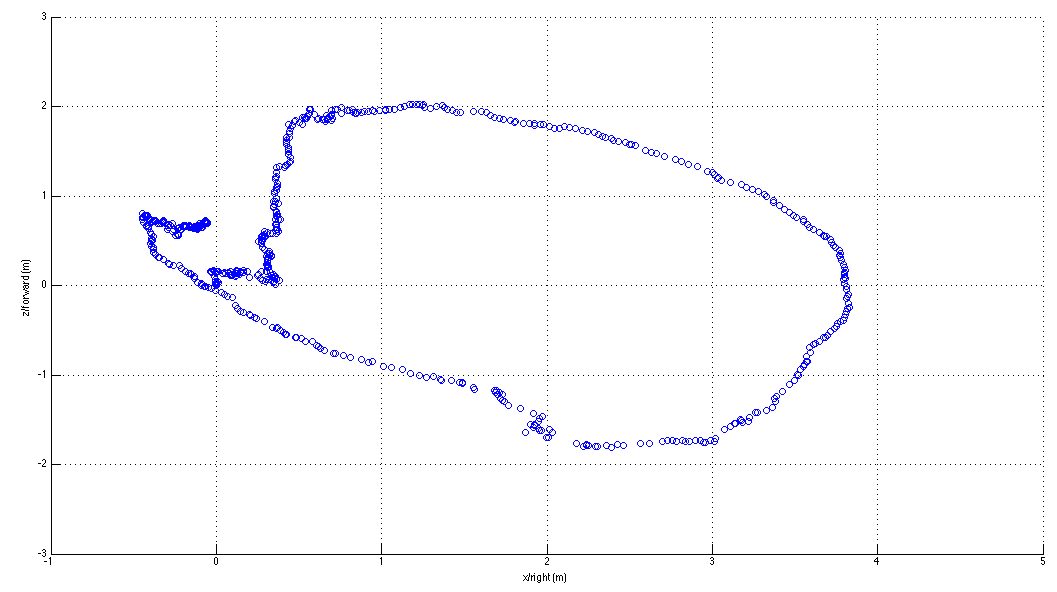
\includegraphics[width=0.4\textwidth]{trajtop.png}
		\label{trajtop}
	}
	\caption{The trajectory generated with incremental rotations and translations}
	\label{traj}
\end{figure}

\begin{figure}[t!]
	\centering
	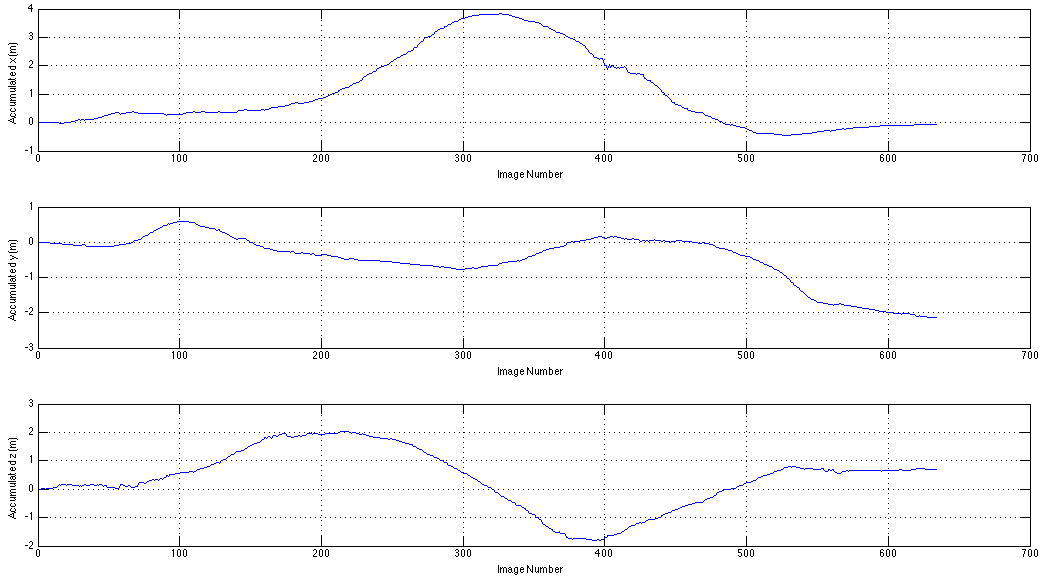
\includegraphics[width=0.8\textwidth]{position_adjusted.png}
	\caption{Camera Positions from Concatenated Transformations}
	\label{pos}
\end{figure}

\begin{figure}[t!]
	\centering
	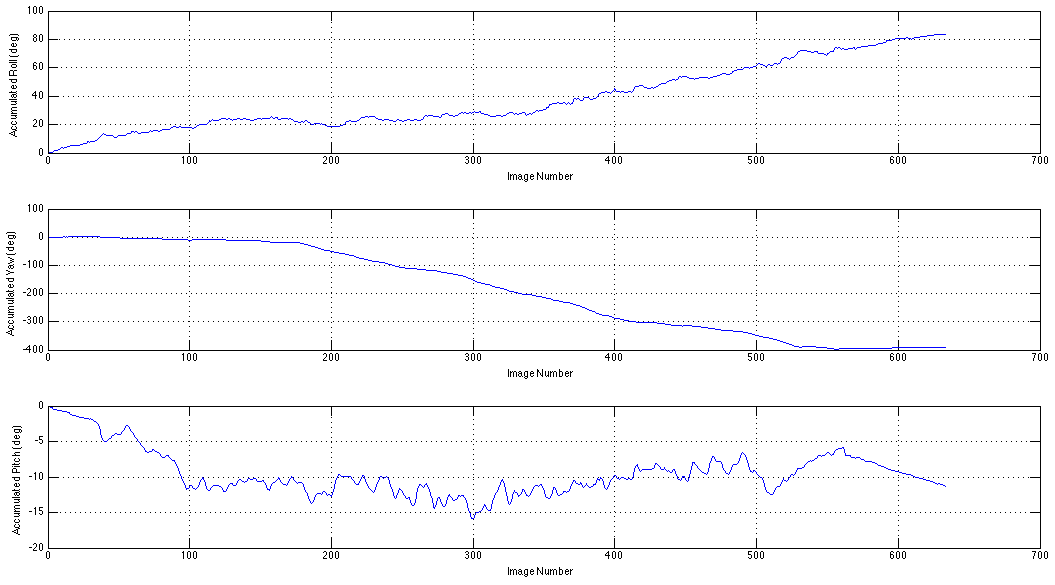
\includegraphics[width=0.8\textwidth]{orientation.png}
	\caption{Camera Orientations (ZYX) from Concatenated Transformations}
	\label{orient}
\end{figure}

\item % f
Part (e) was repeated with different RANSAC numbers of iterations and thresholds.
\begin{itemize}
\item Decrease the number of iterations by a factor of 10:

The trajectory is shown in Figure \ref{traj_iter} and the position and orientation plots are shown in Figures \ref{pos_iter} and \ref{orient_iter}. The decrease in the number of iterations resulted in additional drifts due to less optimal camera matrix estimations.

\begin{figure}[h!]
	\centering
	\subfloat[Front view]{
		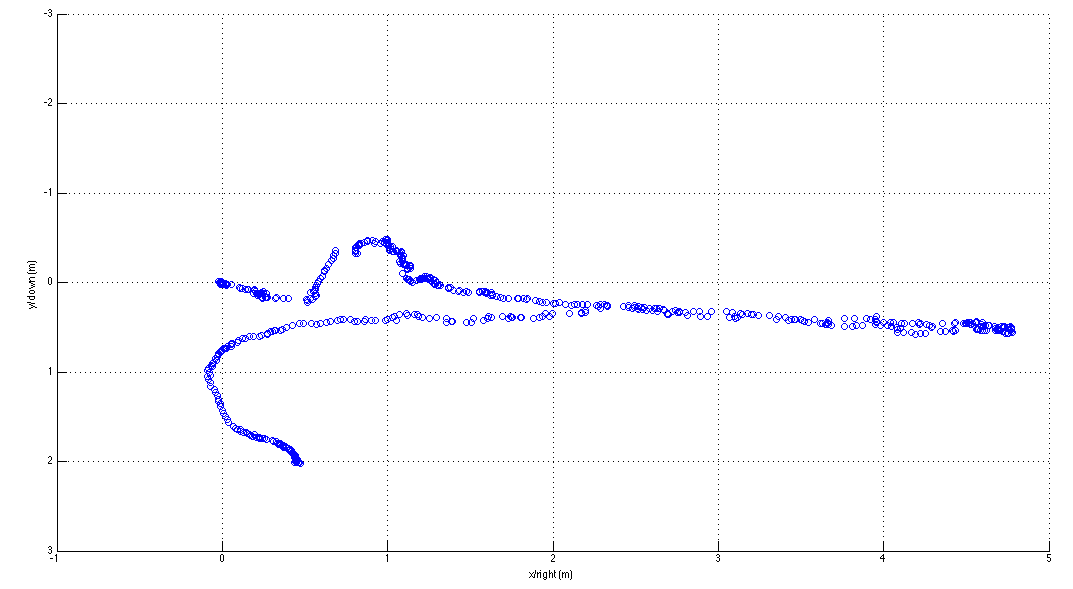
\includegraphics[width=0.4\textwidth]{trajside_iter.png}
		}	
	\subfloat[Top view]{
		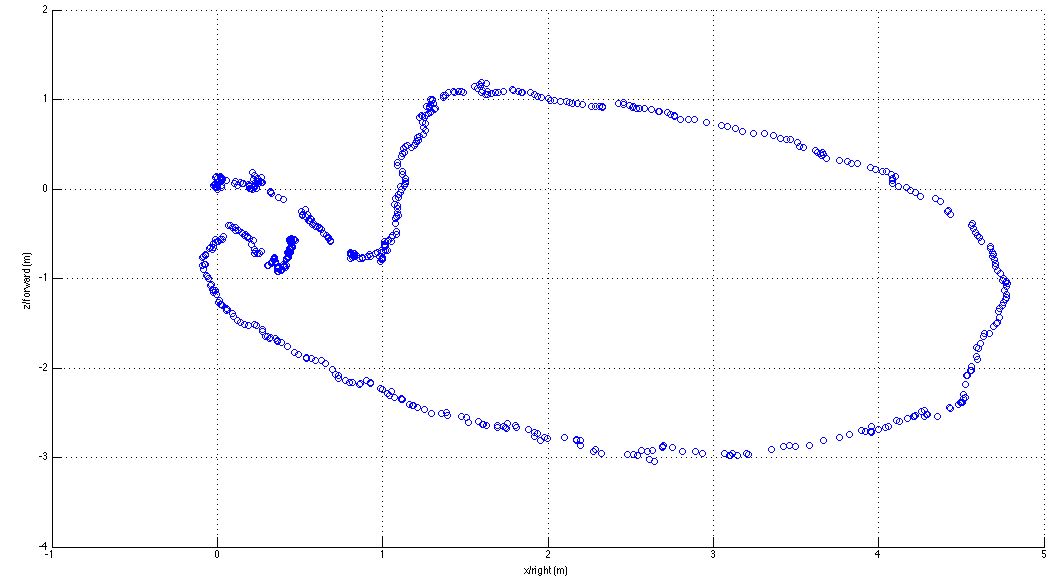
\includegraphics[width=0.4\textwidth]{trajtop_iter.png}
	}
	\caption{The trajectory generated with 10 times fewer RANSAC iterations.}
	\label{traj_iter}
\end{figure}

\begin{figure}[h!]
	\centering
	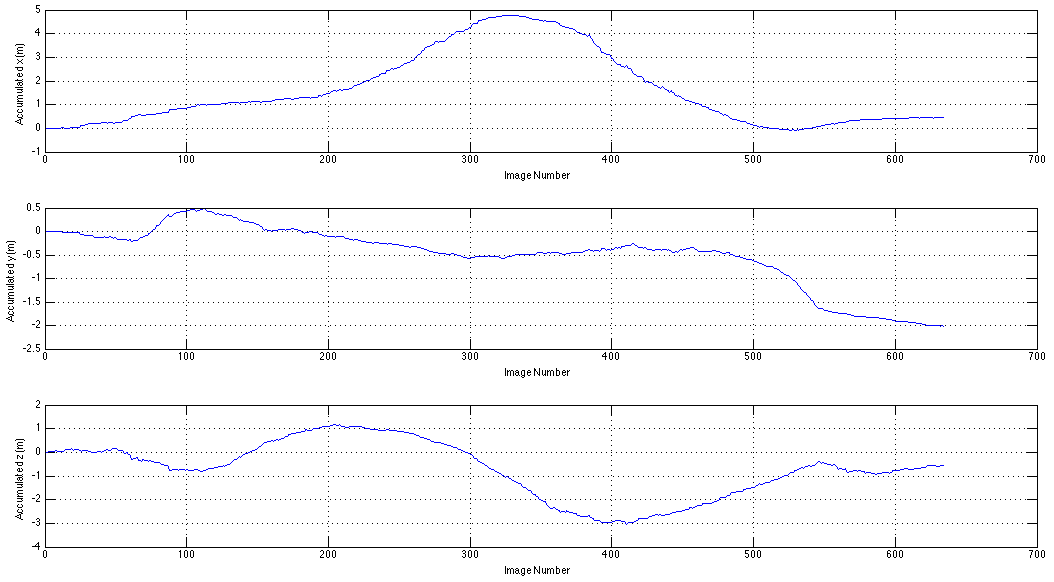
\includegraphics[width=0.8\textwidth]{position_adjusted_iter.png}
	\caption{Camera Positions with 10 times fewer RANSAC iterations.}
	\label{pos_iter}
\end{figure}

\begin{figure}[h!]
	\centering
	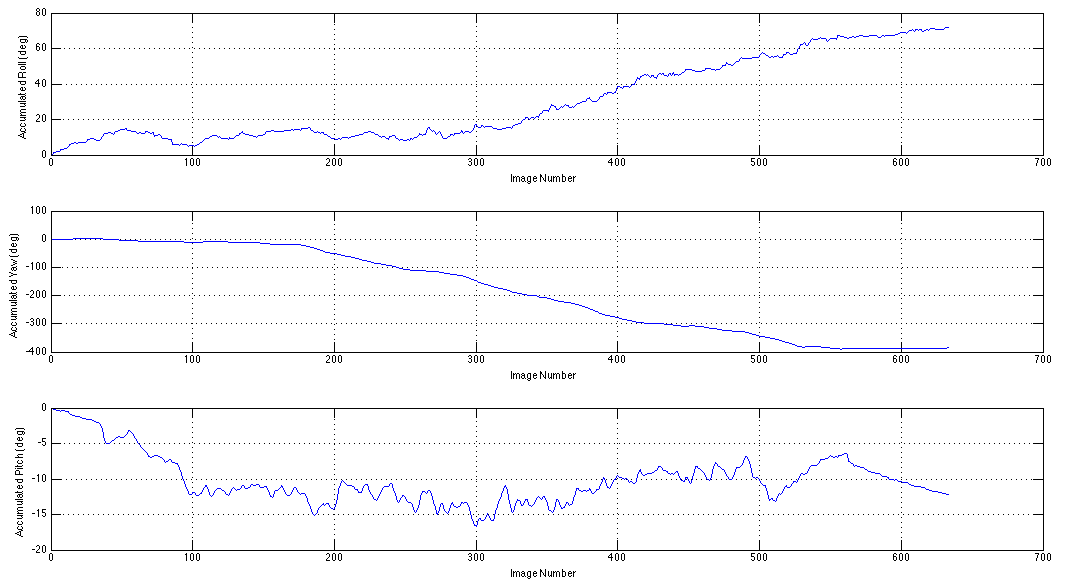
\includegraphics[width=0.8\textwidth]{orientation_iter.png}
	\caption{Camera Orientations with 10 times fewer RANSAC iterations.}
	\label{orient_iter}
\end{figure}

\item Increase the threshold by a factor of 10:

The trajectory is shown in Figure \ref{traj_thres} and the position and orientation plots are shown in Figures \ref{pos_thres} and \ref{orient_thres}. A larger threshold potentially allowed outliers to be included as inliers during the RANSAC routine, thus yielding less optimal and noisier camera matrix estimations. As a result, additional errors in drift were introduced to the trajectory.

\end{itemize}

\begin{figure}[h!]
	\centering
	\subfloat[Front view]{
		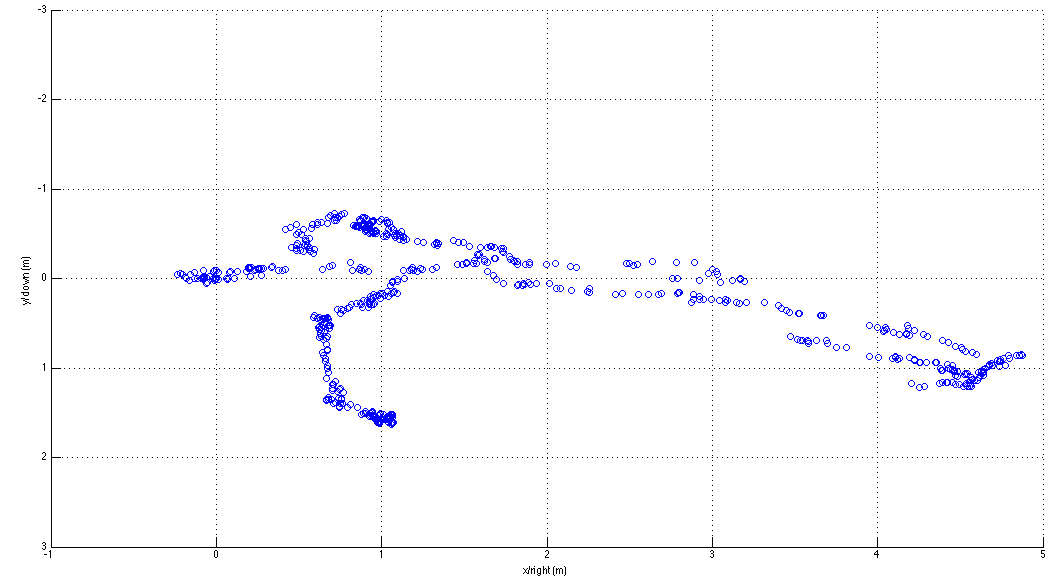
\includegraphics[width=0.4\textwidth]{trajside_thres.png}
	}
	\subfloat[Top view]{
		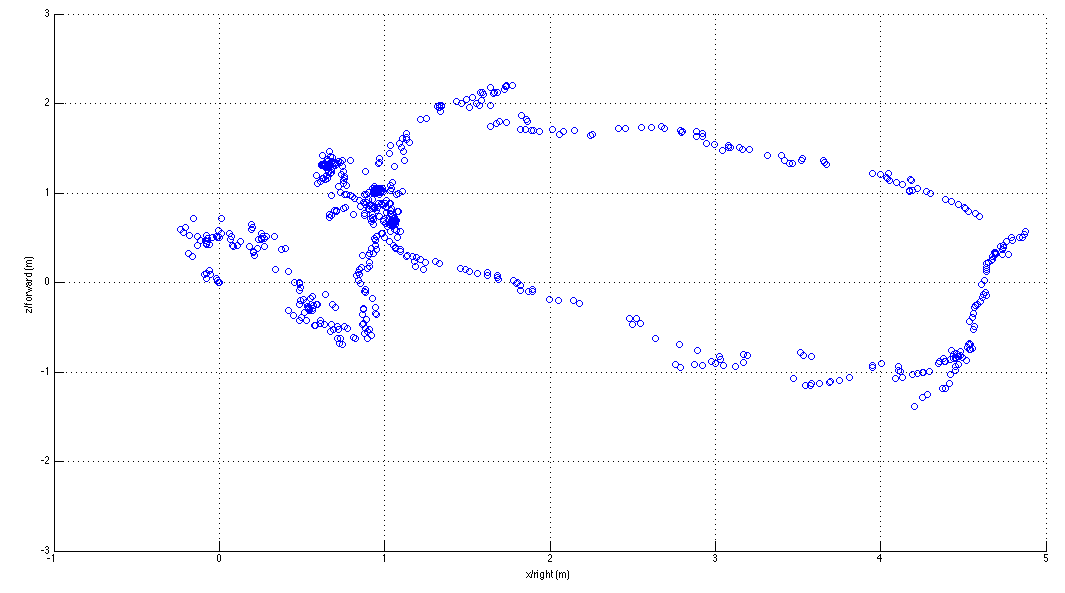
\includegraphics[width=0.4\textwidth]{trajtop_thres.png}
	}
	\caption{The trajectory generated with 10 times RANSAC threshold.}
	\label{traj_thres}
\end{figure}
\begin{figure}[h!]
	\centering
	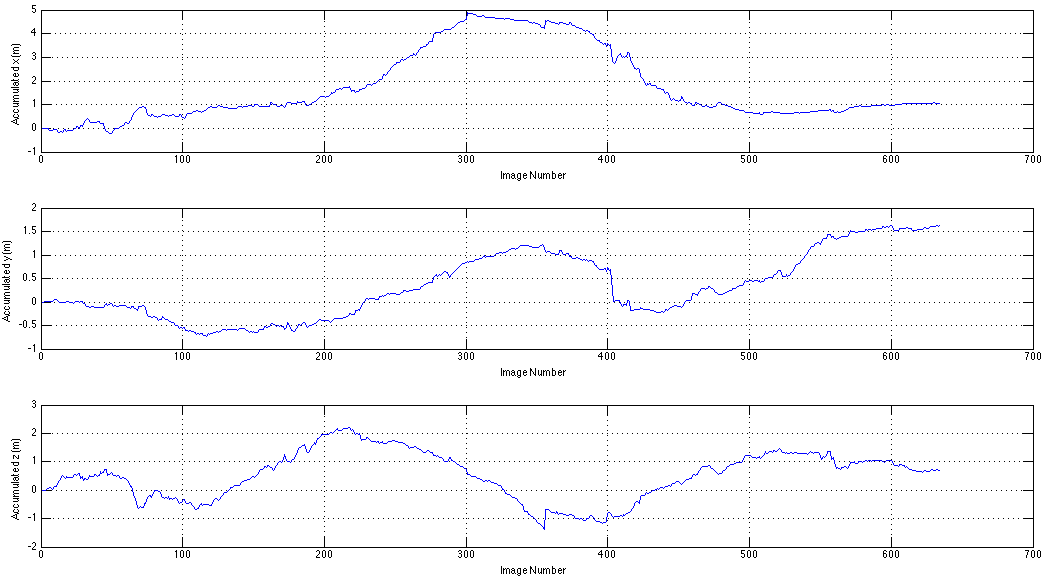
\includegraphics[width=0.79\textwidth]{position_adjusted_thres.png}
	\caption{Camera Positions with 10 times RANSAC threshold.}
	\label{pos_thres}
\end{figure}
\begin{figure}[h!]
	\centering
	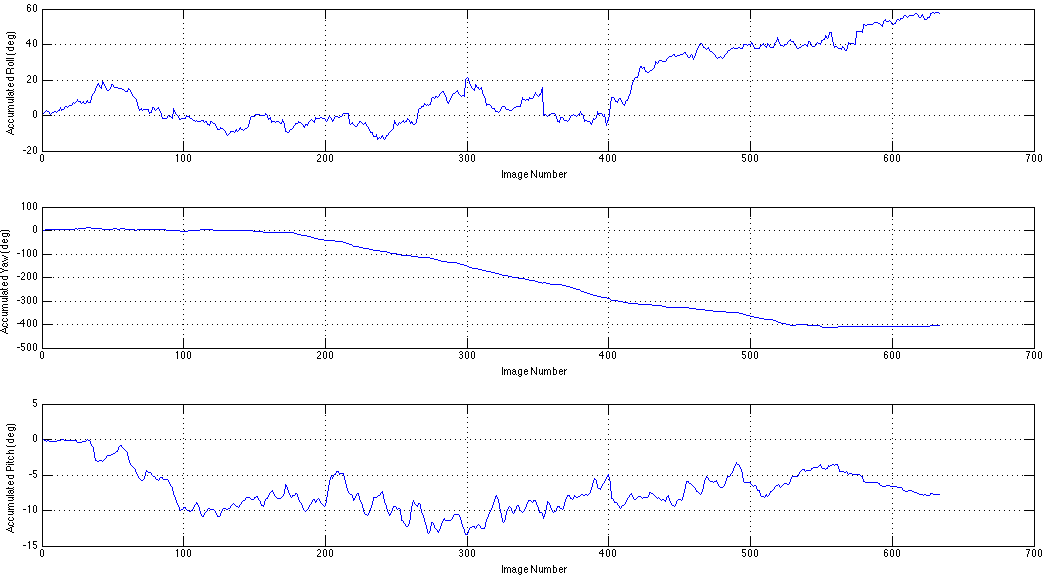
\includegraphics[width=0.79\textwidth]{orientation_thres.png}
	\caption{Camera Orientations with 10 times RANSAC threshold.}
	\label{orient_thres}
\end{figure}

\newpage 
\item % g
The trajectory computed did not return exactly to the starting position (see Figure \ref{trajtop}). As seen in Figure \ref{trajfront}, the height of the final position was even below ground level. This drift could be explained by the accumulated errors in estimations across each pair of successive frames. After hundreds of estimations, the errors became observably significant in the position estimates. Figures \ref{pos_drift} and \ref{orient_drift} display the "drift profile" in position and orientation obtained by calculating the estimation errors between each image frame and its own.

Knowing that such drift was proportional to the image frames calculated, a new trajectory was generated using only every seven frames, as shown in Figure \ref{traj_int7}. The position and orientation are shown in Figure \ref{pos_int7} and \ref{orient_int7}. This interval of seven images was determined empirically. Intuitively, a smaller interval would account for more image drifts while a larger interval would start to exhibit unstable estimations due to drastic scene (and hence, features) changes.

\begin{figure}[h!]
	\centering
	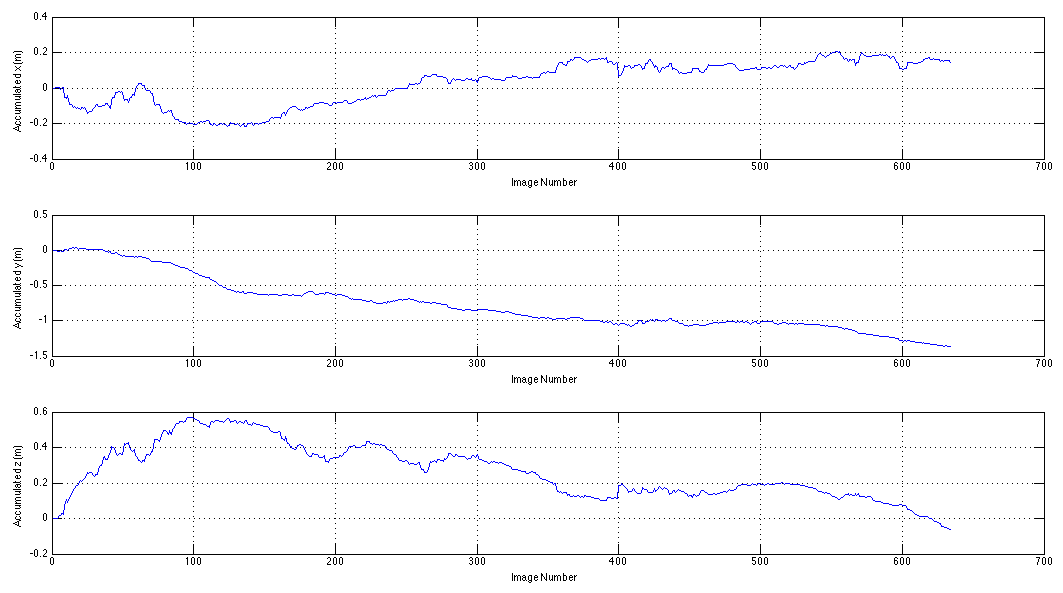
\includegraphics[width=0.75\textwidth]{position_drift.png}
	\caption{Position Drift Across All Successive Images}
	\label{pos_drift}
\end{figure}

\begin{figure}[h!]
	\centering
	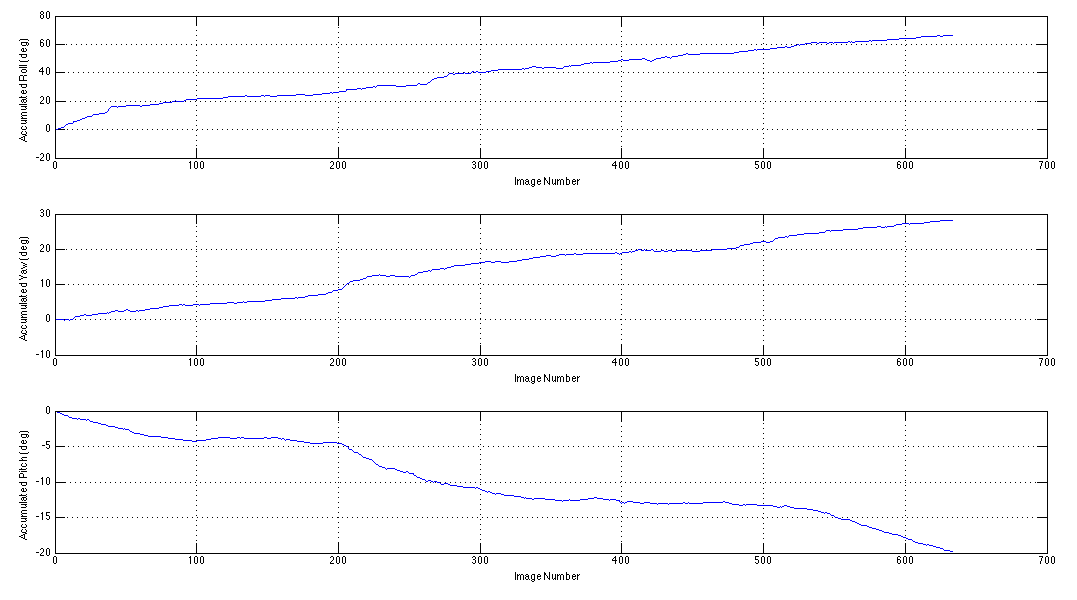
\includegraphics[width=0.75\textwidth]{orientation_drift.png}
	\caption{Orientation Drift Across All Successive Images}
	\label{orient_drift}
\end{figure}

\begin{figure}[h!]
	\centering
	\subfloat[Front view.]{
		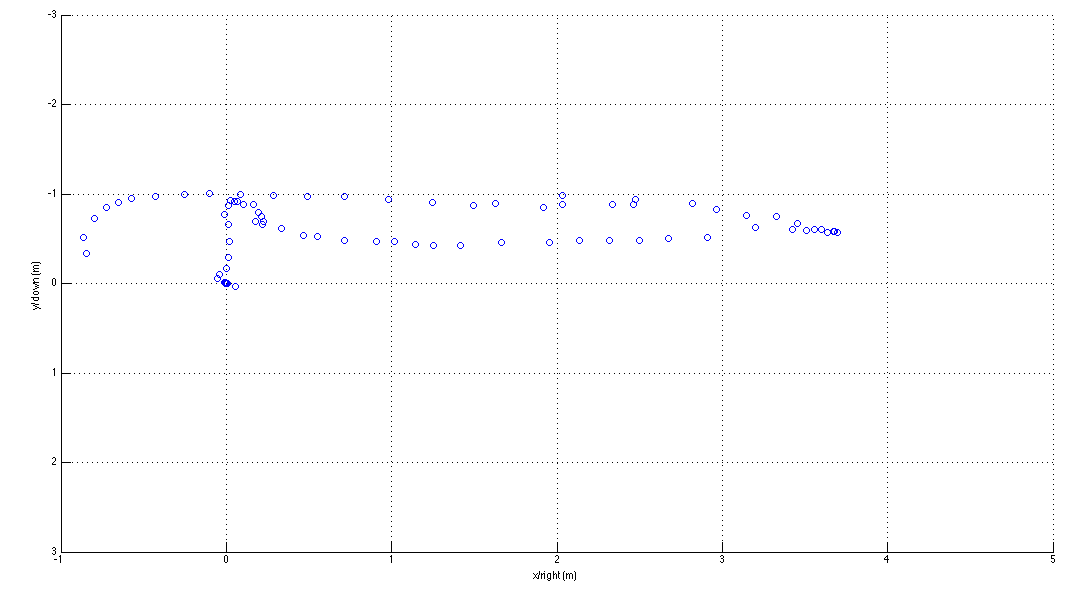
\includegraphics[width = 0.4\textwidth]{trajside_int7.png}
	}
	\subfloat[Top view.]{
		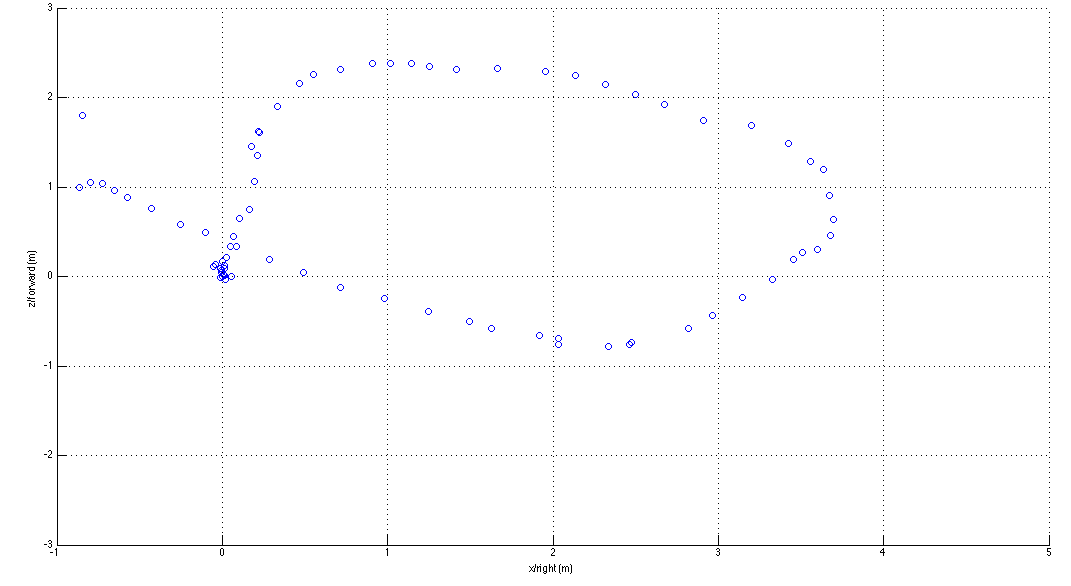
\includegraphics[width = 0.4\textwidth]{trajtop_int7.png}
	}
	\caption{The trajectory generated with every seven images}
	\label{traj_int7}
\end{figure}

\begin{figure}[h!]
	\centering
	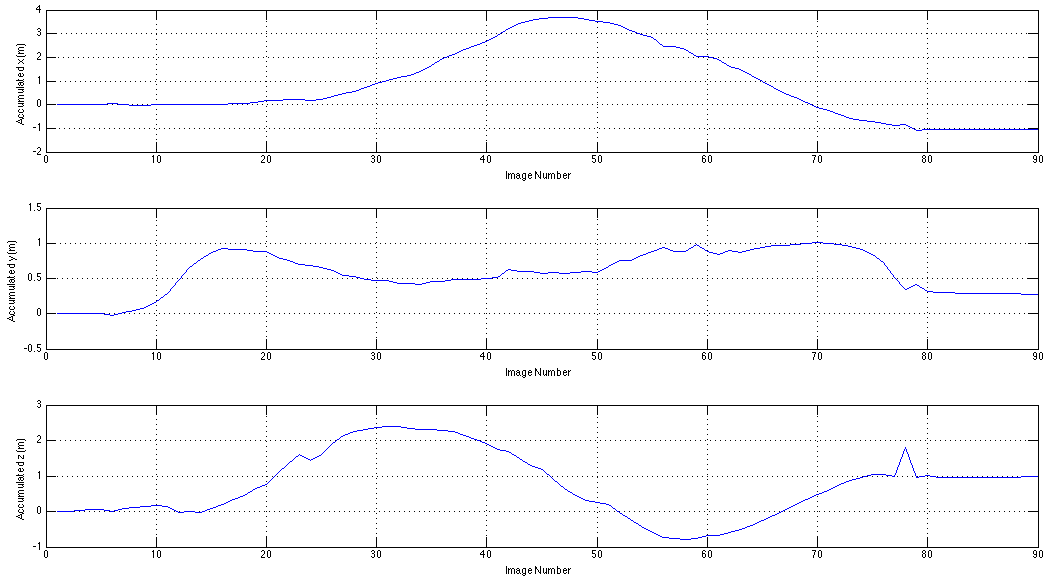
\includegraphics[width=0.79\textwidth]{position_adjusted_int7.png}
	\caption{Camera Positions with every seven images}
	\label{pos_int7}
\end{figure}

\begin{figure}[h!]
	\centering
	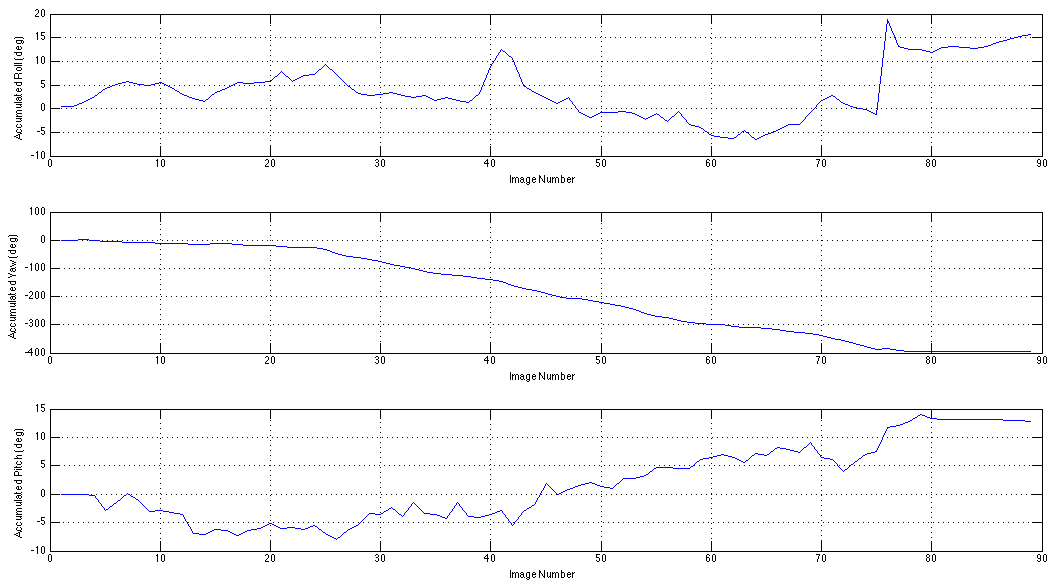
\includegraphics[width=0.79\textwidth]{orientation_int7.png}
	\caption{Camera Orientations with every seven images}
	\label{orient_int7}
\end{figure}

\end{enumerate}

\section{Unscented Kalman Filter}

Presented here are four sets of our Unscented Kalman filter results. Figure  \ref{baseline}
 shows the result of our baseline test, in which all the noise covariances are set as 0.001. To demonstrate the effects of changing the initial noise sigma, IMU noise and observation noise, we have made changes to each group of sigma values to make them much larger than the baseline. 
 
Figure \ref{highi} shows the filter output when the initial noise sigma is increased by 100 times. A large error is observed initially, but it then tracks properly after several seconds. Note that the filter needs longer time to reduce the estimation error for some fast-changing states ($z$ in this case).
In Figure \ref{highq}, the IMU noise is increased by 50 times. Larger IMU noise and bias noise will result in increased filter error in the Model Update process; however, it will be corrected by the observations in the Correction process. In conclusion, adding IMU noise will make the filter output noisy, without creating a large bias. 

\begin{figure}[b!]
	\centering
	\subfloat[][$x$]{\includegraphics[width=0.24\linewidth]{b_x.eps}}
	\subfloat[][$y$]{\includegraphics[width=0.24\linewidth]{b_y.eps}}	
	\subfloat[][$z$]{\includegraphics[width=0.24\linewidth]{b_z.eps}}
	\subfloat[][Yaw]{\includegraphics[width=0.24\linewidth]{b_yaw.eps}}	
	\caption{Baseline results with all parameters set to 0.001.}
	\label{baseline}
\end{figure}
\begin{figure}[b!]
	\centering
	\subfloat[][$x$]{\includegraphics[width=0.24\linewidth]{i_x.eps}}
	\subfloat[][$y$]{\includegraphics[width=0.24\linewidth]{i_y.eps}}	
	\subfloat[][$z$]{\includegraphics[width=0.24\linewidth]{i_z.eps}}
	\subfloat[][Yaw]{\includegraphics[width=0.24\linewidth]{i_yaw.eps}}	
	\caption{Results with 100 times initial noise coefficients.}
	\label{highi}
\end{figure}
\begin{figure}[b!]
	\centering
	\subfloat[][$x$]{\includegraphics[width=0.24\linewidth]{q_x.eps}}
	\subfloat[][$y$]{\includegraphics[width=0.24\linewidth]{q_y.eps}}	
	\subfloat[][$z$]{\includegraphics[width=0.24\linewidth]{q_z.eps}}
	\subfloat[][Yaw]{\includegraphics[width=0.24\linewidth]{q_yaw.eps}}	
	\caption{Results with 50 times IMU noise coefficients.}
	\label{highq}
\end{figure}

\begin{figure}[h]
	\centering
	\subfloat[][$x$]{\includegraphics[width=0.24\linewidth]{r_x.eps}}
	\subfloat[][$y$]{\includegraphics[width=0.24\linewidth]{r_y.eps}}	
	\subfloat[][$z$]{\includegraphics[width=0.24\linewidth]{r_z.eps}}
	\subfloat[][Yaw]{\includegraphics[width=0.24\linewidth]{r_yaw.eps}}	
	\caption{Results with 100 times observation noise coefficients.}
	\label{highr}
\end{figure}

Figure \ref{highr} shows the filter output when the observation noise is increased by 100 times. Note that there is no noticeable noise, but bias and degraded accuracy are observed. This is because a wrong observation will lead to a bias correction that affects all the state vectors. 

Table \ref{np} shows the noise parameters. The observation noise is estimated by computing the mean and covariance of a series of data derived by subtracting the ground truth\footnote{This is later considered to be inappropriate. These parameters have been re-estimated using the data collected from when the drone is stationary on the ground. In this
period of time, the observation is thought to be pure noise. 
} from the observation. The IMU bias noise is given as 0.03. The acceleration and angular velocity noises are estimated by computing their covariances when the drone is in a relatively stationary state. The initial sigma value has been manually tuned: it appears that as long as the initial values are kept within a reasonable range, the result 
will not be affected too much. The filter output after noise parameter tuning is shown in Figure \ref{tuning}.

\begin{table}[h]
	\centering	
	\caption{Noise Parameters}	\label{np}\vspace{-6pt}
	\begin{tabular}{llll} \toprule
	{\tt init\_pos\_sigma}    & 0.01    & {\tt sigma\_bw}           & 0.03      \\
	{\tt init\_rpy\_sigma}    & 0.001   &  {\tt sigma\_a}            & 0.08      \\
	{\tt init\_vel\_sigma}    & 0.001    &  {\tt sigma\_ba}           & 0.03    \\
	{\tt init\_bw\_sigma}    & 0.001    &  {\tt sigma\_xy}           & 0.077     \\
	{\tt init\_ba\_sigma}     & 0.001      &  {\tt sigma\_z}            & 0.05  \\
	{\tt sigma\_w}            & 0.03       & {\tt sigma\_ yaw}           & 0.02  \\ \bottomrule
	\end{tabular}
\end{table}

\begin{figure}[t]
	\centering
	\subfloat[][$x$]{\includegraphics[width=0.24\linewidth]{r_x.eps}}
	\subfloat[][$y$]{\includegraphics[width=0.24\linewidth]{r_y.eps}}	
	\subfloat[][$z$]{\includegraphics[width=0.24\linewidth]{r_z.eps}}
	\subfloat[][Yaw]{\includegraphics[width=0.24\linewidth]{r_yaw.eps}}	
	\caption{Results with tuned noise parameters}
	\label{tuning}
\end{figure}

Figure \ref{MSE} shows the mean square error and its distribution for the observed position against the ground truth. It can be seen from the distribution that after tuning the noise parameter, the largest mean square error is 0.013. The mean error is 0.0008, with most of the errors below 0.004.

\begin{figure}[t!]
	\centering
	\subfloat[][Mean Square Error Over Time]{\includegraphics[width=0.32\textwidth]{MSE.eps}}\quad
	\subfloat[][Error Distribution]{\includegraphics[width=0.32\textwidth]{MSE_dist.eps}}
	\caption{Position Estimation Error}
	\label{MSE}	
\end{figure}

\begin{figure}[t!]
	\centering
	\subfloat[][Position]{\includegraphics[width=0.32\textwidth]{MSE_t.eps}}\quad
	\subfloat[][$x$]{\includegraphics[width=0.32\textwidth]{MSE_x.eps}}\\
	\subfloat[][$y$]{\includegraphics[width=0.32\textwidth]{MSE_y.eps}}\quad
	\subfloat[][$z$]{\includegraphics[width=0.32\textwidth]{MSE_z.eps}}	
	\caption{Position Error and their Distributions}
	\label{MSEinterval}	
\end{figure}

The data from 15s to 20s have been selected to compare the empirical standard deviation and to estimate the UKF 1-sigma. Figure \ref{MSEinterval} shows the position errors and their distributions. The empirical standard deviations in this time interval are: {\tt std\_x}: 0.026569, {\tt std\_y}: 0.015594, {\tt std\_z}: 0.016420. The estimated 1-sigma values are $x$: 0.030517, $y$: 0.030510, $z$: 0.014851. The empirical standard deviation is smaller than the estimation. This is because the noise of each estimation state will be propagated to the next state. When updating the state, the noise will be accumulated, but the mean state value will generally stay close to the ground truth. In another word, UKF estimates the noise in the process update in a conservative way, resulting in a larger estimated standard deviation than the empirical standard deviation.

\vfill
\begin{center}
	
\includegraphics[scale = 0.4]{evolutus-black.eps}
\end{center}


\thispagestyle{fancy}
	
\end{onehalfspacing}
\end{document} 